\label{s:discussion}

\begin{itemize}
\item Combining first and second derivatives: firsts are good at edges, seconds are good at line centres - they complement each other.

\item Discussion about linear regression coefficients: how they take a sinusoidal appearance, how we need to choose between two discrete orientations (which is not possible with a `vanilla' linear regressor)
%
\begin{figure}[t]
	\centering
		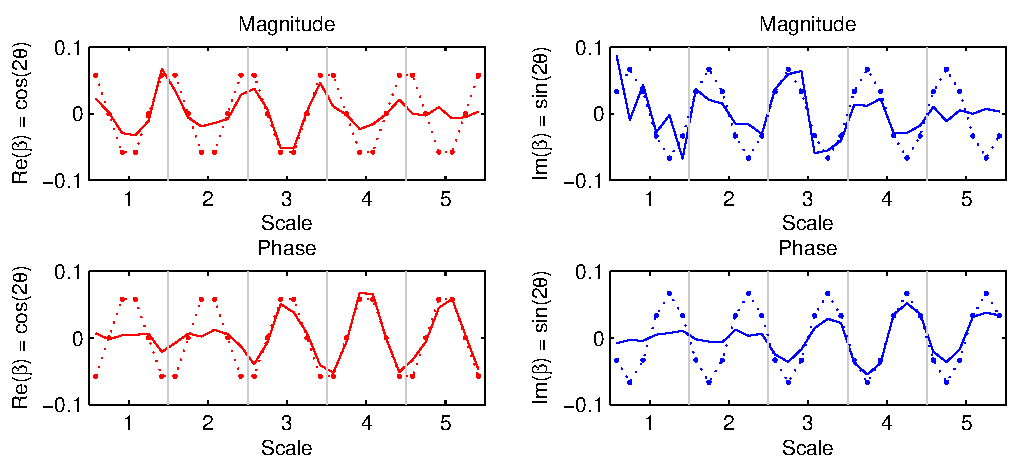
\includegraphics[width=0.9\columnwidth]{\figpath/linreg_coeffs}
	\caption{Linear regression coefficients for (left) $\cos 2\theta$ and (right) $\sin 2\theta$, using (top) response magnitude and (bottom) response phase.}
	\label{f:linreg_coeffs}
\end{figure}
%
\item Logistic regression can be used to limit the output to -1..+1. Boosted regression implicitly does the same by predicting only what it has seen before. These limits, however, are applied to sinT and cosT independently which means you can still get values outside of the unit circle.

\item Random Forest classifier/regressor has lots of details to get right, not least in making sure that the orientations wrap around correctly. Also differences in how the branches are split etc.
\end{itemize}

The results of our experimental evaluation are extremely encouraging, and represent a significant improvement over the current state of the art.

Although learning accounts for a significant part of this improvement, the choice of representation is also important and will have a different effect on performance depending on the task in hand. For example, constructing a representation based on the raw responses to Linop filters produces features that are excellent for estimating structure orientation but provide less information for determining structure shape and thus type.

Conversely, features formed from the monogenic signal are good at determining structure type - most likely because of the inclusion of the phase measure - while they perform relatively poorly at detection and orientation estimation.

For these reasons, it seems fair to conclude that the \dtcwt{} provides the best all round representation. It produced the strongest performance for all three tasks (curvilinear structure detection, orientation estimation and spicule classification). Moreover, the \dtcwt{} incurs the least overhead when working with full-size real images that require block-wise classification/regression. For example, initial tests show that the structure detection and orientation regression can be performed on a full-size (approximately $3000 \times 2400$ pixels) mammogram in approximately 1hr 30mins.

We show that, overall, our approach is significantly better than the current state-of-the-art, and that we can distinguish effectively between curvilinear structures associated with malignancy (spicules) and those associated with normal structure (vessels, ducts etc).




We have presented a discriminative learning-based approach to the detection and classification of curvilinear structures, based on a combination of \dtcwt{} representation of local structure and random forest classification. We have applied the method to the challenging problem of detecting and estimating the orientation of curvilinear structures in mammograms and distinguishing between normal and abnormal structures. The results of our experimental evaluation are extremely encouraging, and represent a significant improvement over the current state of the art.

We have also introduced learning-based variants of three existing methods, demonstrating that whilst learning accounts for a significant part of this improvement, the choice of representation is also important and will have a different effect on performance depending on the task in hand. For example, constructing a representation based on the raw responses to Linop filters produces features that are excellent for estimating structure orientation but provide less information for determining structure shape and thus type. Conversely, features formed from the monogenic signal are good at determining structure type - most likely because of the inclusion of the phase measure - whilst they perform relatively poorly at detection and orientation estimation. For these reasons, it seems fair to conclude that the \dtcwt{} provides the best all round representation. It produced the strongest performance for all three tasks (curvilinear structure detection, orientation estimation and spicule classification). Moreover, as discussed in section 5.2, of all the methods, the DT-CWT incurs the least overhead when working with full-size real images that require block-wise classification/regression. For example, initial tests show that the structure detection and orientation regression can be performed on a full-size (~3000 x 2400 pixels) mammogram in ~1hr 30mins.

Our next goal is to show that improving the individual steps of curvilinear structure and orientation estimation result in a subsequent improvement for a high level task such as detecting patterns of spiculations indicative of disease. Moreover we hope to show that classification into structure type can further aid such tasks by focusing only (or at least more) on those structures most likely to be associated with disease. 